\startappendix{Sample Mechanisms and Features}
\label{chapter:appendix_features}

Sample enabling mechanisms and features of the conceptual framework for information discovery and curation are presented in Table~\ref{table:features}.
\begin{longtable}{|p{0.90\linewidth}|}
\caption{Navigation Samples}\label{table:features}\\
\hline
\textbf{Descriptional Navigation} 		\\	
\\
\underline{Search-based navigation}	\\	
YELP (www.yelp.ca)\\	

\includegraphics[width=\linewidth]{search.png}\\
\\
\underline{Integrated search}				\\
SHOPSTYLE (www.shopstyle.ca)\\

\includegraphics[width=\linewidth]{integrated_search.png}\\
\\
\hline
\pagebreak
\hline
\textbf{Referential Navigation}       		\\
\\
\underline{Categories}		\\	
PINTEREST (www.pinterest.com)	\\ 		
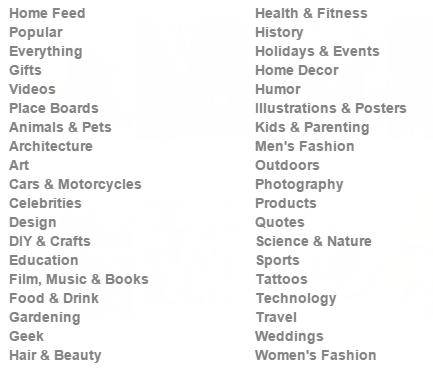
\includegraphics[width=0.7\linewidth]{categories.png}\\
\\
\underline{Facets}				    		\\
ROTTEN TOMATOES (www.rottentomatoes.com)\\

\includegraphics[width=0.4\linewidth]{facets.png}\\
\\
\hline
\pagebreak
\hline
\underline{Filters}					  		\\
YELP (www.yelp.ca)\\
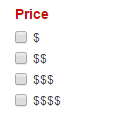
\includegraphics[width=0.3\linewidth]{filters.png}\\

\underline{Tags}\\
FLICKR (www.flickr.com)				      		\\
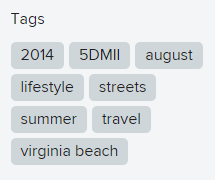
\includegraphics[width=0.3\linewidth]{tags.png}\\
\\
\underline{Search by item or resource}		\\
TRIPADVISOR (www.tripadvisor.ca)\\

\includegraphics[width=0.3\linewidth]{resource.png}\\

\\
\underline{Integrated reference}			\\
GOOGLEMAPS (www.google.ca/maps)\\
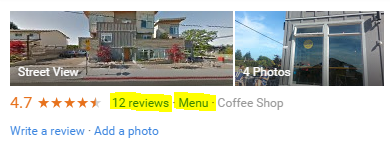
\includegraphics[width=0.8\linewidth]{integrated_reference.png}\\
\hline

\pagebreak
\hline

\textbf{Opportunistic Navigation}          \\
\\
\underline{Opportunistic navigation mechanism}        \\
WIKIPEDIA (en.wikipedia.org)\\
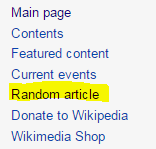
\includegraphics[width=0.3\linewidth]{opportunistic.png}\\
\\
\underline{Integrated opportunistic navigation} \\ 
STUMBLEUPON (www.stumbleupon.com)\\

\includegraphics[width=0.5\linewidth]{integrated_opportunistic.png}\\
\\
\hline        
\textbf{System-regulated Navigation}            \\	
\\	
\underline{Static direct display}           \\
WE HEART IT (weheartit.com)\\
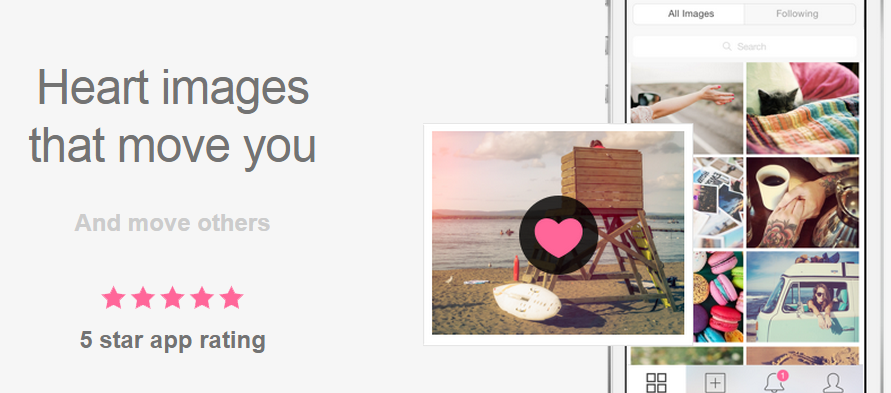
\includegraphics[width=\linewidth]{static_display.png}\\
\\
\hline
\pagebreak
\hline
\underline{Featured content}             	\\
IMDB (www.imdb.com)\\
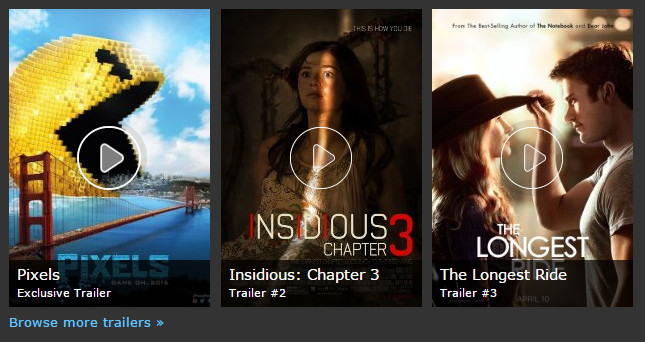
\includegraphics[width=\linewidth]{featured.png}\\
\\
\underline{News feed}      			\\
TRIPADVISOR (www.tripadvisor.ca)\\
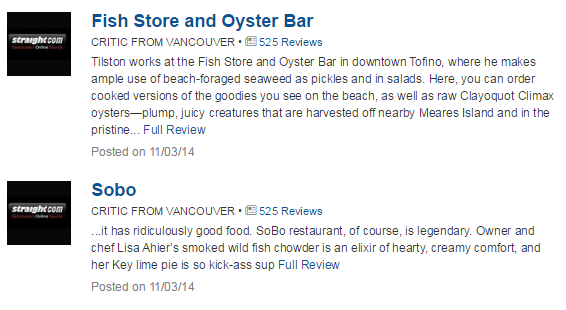
\includegraphics[width=0.7\linewidth]{news.png}\\
\hline

\end{longtable}
\clearpage

\begin{longtable}{|p{0.90\linewidth}|}
\caption{Exploration Samples}\\

\hline
\textbf{Visual and textual cues of multiple resources}  \\
\\
\underline{Visual preview}                 \\
YOUTUBE (www.youtube.com)\\
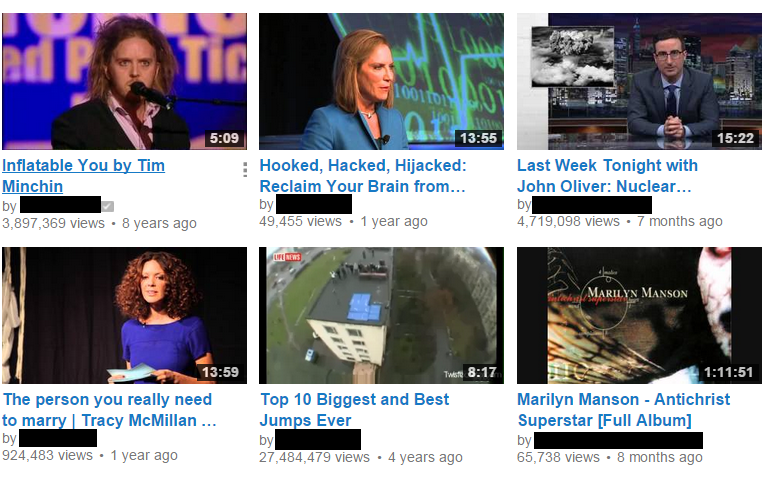
\includegraphics[width=0.8\linewidth]{visual_previews.png}\\
\\
\underline{Textual preview} \\
SCOOP.IT! (www.scoop.it)\\
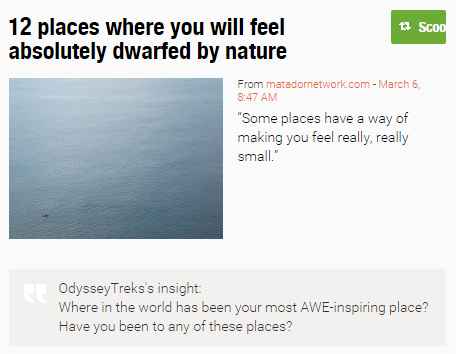
\includegraphics[width=0.8\linewidth]{textual_preview.png}\\
\\
\hline
\pagebreak
\hline
\textbf{Visual and textual cues of a single resource} \\
\\
\underline{Visual cues}                  \\
TRIPADVISOR (www.tripadvisor.ca)\\
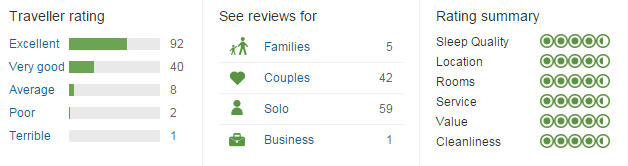
\includegraphics[width=\linewidth]{visual_cue.png}\\
\\

\underline{Textual cues}                 \\
GOOGLE MAPS (www.google.ca/maps)\\

\includegraphics[width=0.6\linewidth]{textual_cue.png}\\
\\
\hline
\textbf{Spatial proximal cues of multiple resources}  \\
\\
\underline{List}  						\\
GOOGLE MAPS (www.google.ca/maps)\\
\includegraphics[width=0.6\linewidth]{list.png}\\
\\
\hline
\pagebreak
\hline
\underline{Grid}   						 \\
VIMEO (vimeo.com)\\
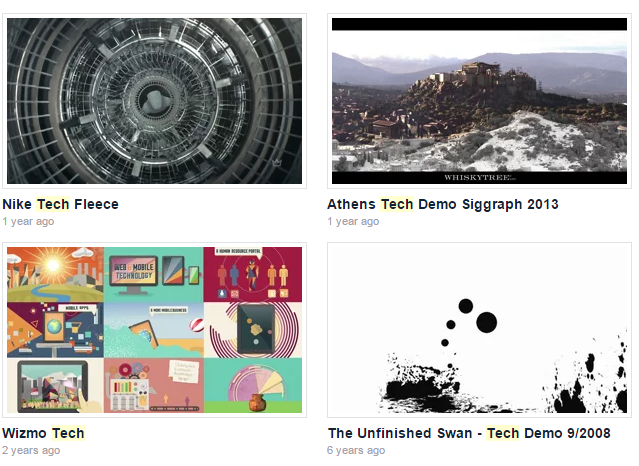
\includegraphics[width=\linewidth]{grid.png}\\
\\
\underline{Gallery}  					\\
TUMBLR (www.tumblr.com)\\
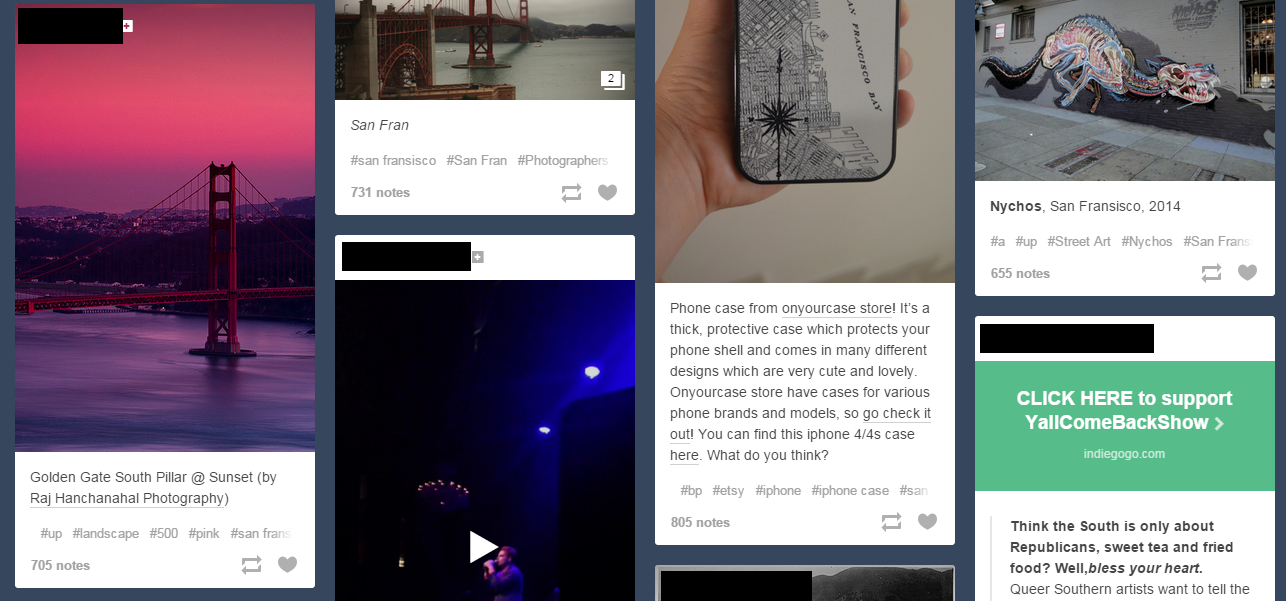
\includegraphics[width=\linewidth]{gallery.png}\\
\hline
\pagebreak
\hline
\underline{Spatial semantic}            \\
GOOGLE MAPS (www.google.ca/maps)\\
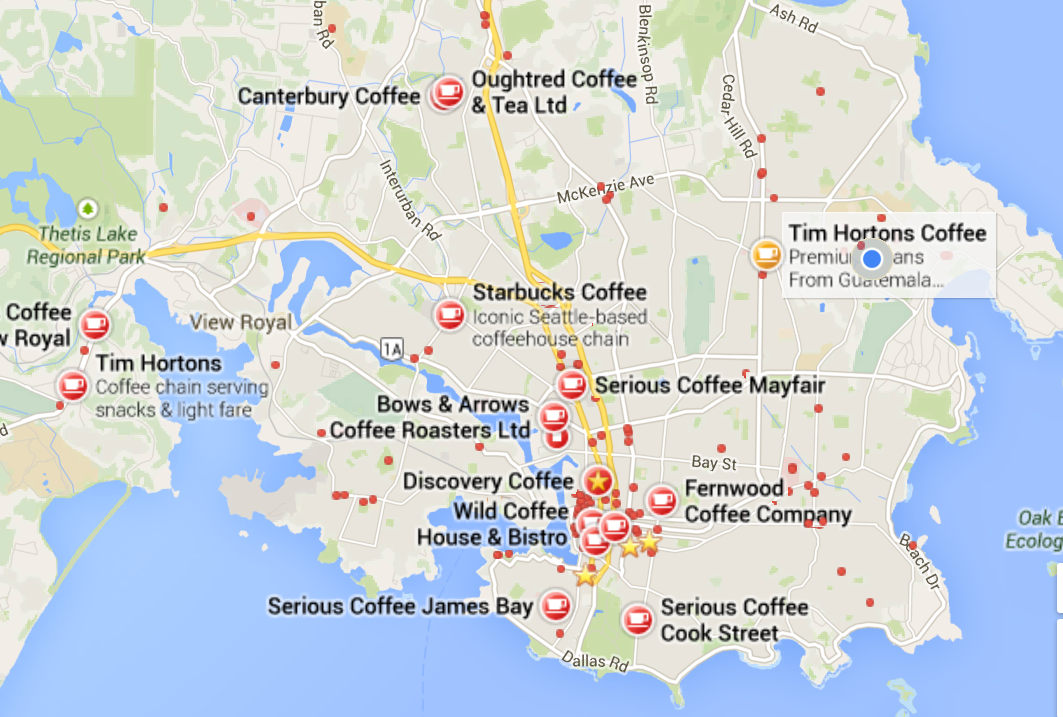
\includegraphics[width=0.6\linewidth]{semantic_multiple.png}\\
\\ 
\textbf{Spatial proximal cues of a single resource} \\
\underline{Spatial semantic}            \\
TRIPADVISOR (www.tripadvisor.ca)\\
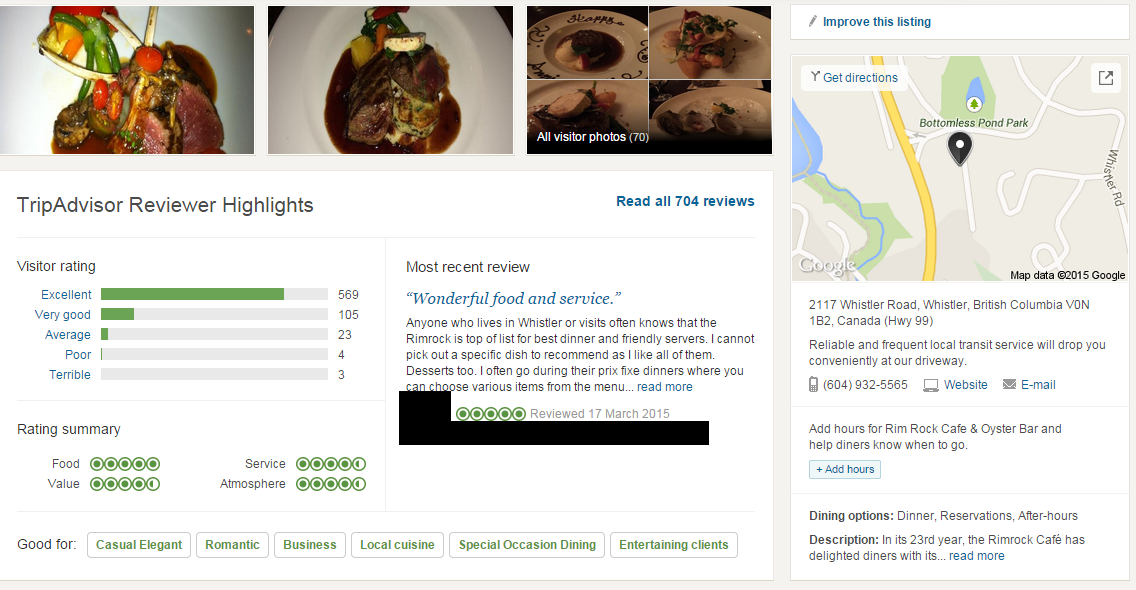
\includegraphics[width=\linewidth]{semantic_single.png}\\
\\
\hline

\end{longtable}
\clearpage
\begin{longtable}{|p{0.90\linewidth}|}
\caption{Curation Samples}\\
\hline

\textbf{Management} \\
\\
\underline{Collection-based categorization}     \\
PINTEREST (www.pinterest.com)\\
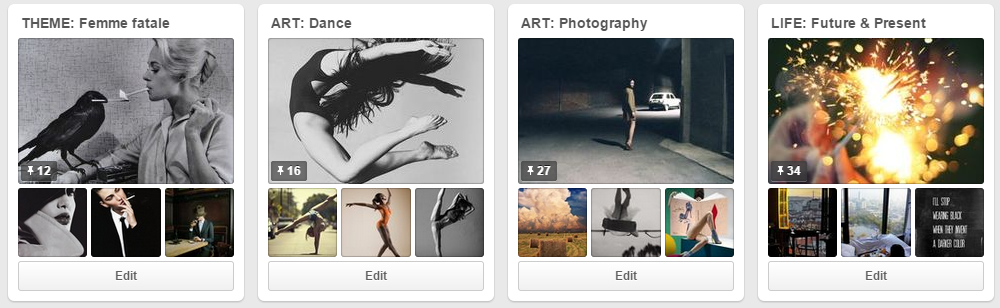
\includegraphics[width=\linewidth]{collection.png}\\
\\
\underline{Tag-based categorization }         \\
TUMBLR (www.tumblr.com)\\
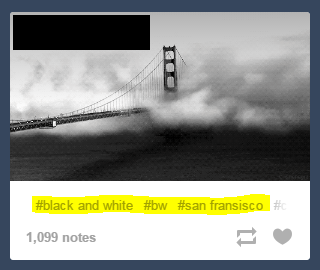
\includegraphics[width=0.4\linewidth]{tagging.png}\\

\\
\hline
\textbf{Preservation} \\
\underline{Internal preservation of internal resources}		\\
BUCKETLIST (bucketlist.org)\\

\includegraphics[width=0.7\linewidth]{internal_internal.png}\\
\\
\hline
\pagebreak
\hline
\underline{Internal preservation of external resources}      \\
PINTEREST (www.pinterest.com)\\
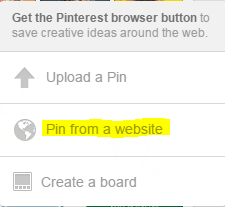
\includegraphics[width=0.4\linewidth]{internal_external.png}\\
\\
\underline{External preservation of internal resources}     \\
BUCKETLIST (bucketlist.org)\\
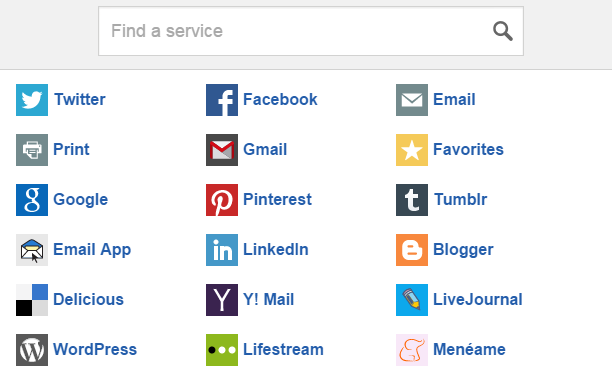
\includegraphics[width=0.7\linewidth]{external_internal.png}\\
\\
\hline
\textbf{Augmentation} \\
\\
\underline{Annotation}  \\ 
YELP (www.yelp.ca)\\
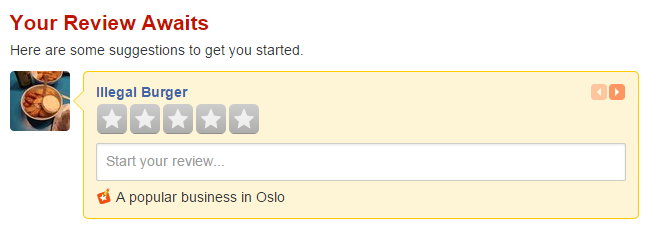
\includegraphics[width=0.7\linewidth]{annotation.png}\\
\hline
\pagebreak
\hline
\underline{Evaluation} \\
YOUTUBE (www.youtube.com)\\
\includegraphics[width=0.4\linewidth]{EVALUATION.png}\\
 \\
\hline  
  
\textbf{Sharing} \\
\\
\underline{Adding resources}         \\
YOUTUBE (www.youtube.com)\\

\includegraphics[width=0.5\linewidth]{adding.png}\\
\\
\underline{Internal sharing}         \\
PINTEREST (www.pinterest.com)\\

\includegraphics[width=0.5\linewidth]{internal_sharing.png}\\
\\ 
\underline{External sharing}        \\ 
YOUTUBE (www.youtube.com)\\
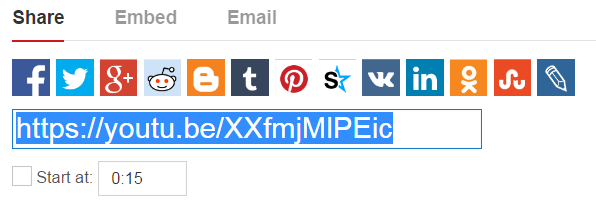
\includegraphics[width=0.9\linewidth]{external_sharing.png}\\
\\
\hline
\pagebreak
\hline  
\textbf{Channel-picking}  	 \\
\\
\underline{User subscription}        \\
FLICKR (www.flickr.com)\\

\includegraphics[width=0.3\linewidth]{user.png}\\
\\
\underline{Site subscription}  	\\
LIFEHACKER (lifehacker.com)\\

\includegraphics[width=0.9\linewidth]{site.png}\\
\underline{Artifact subscription}       \\
PINTEREST (www.pinterest.com)\\
\includegraphics[width=0.3\linewidth]{artifact.png}\\
\\


\hline        

\end{longtable}